\documentclass[conference]{IEEEtran}
\IEEEoverridecommandlockouts
% The preceding line is only needed to identify funding in the first footnote. If that is unneeded, please comment it out.
\usepackage{cite}
\usepackage{amsmath,amssymb,amsfonts}
\usepackage{algorithmic}
\usepackage{graphicx}
\usepackage{textcomp}
\usepackage{xcolor}
\usepackage{multirow}
\usepackage{float}
\usepackage{subfig}
\def\BibTeX{{\rm B\kern-.05em{\sc i\kern-.025em b}\kern-.08em
    T\kern-.1667em\lower.7ex\hbox{E}\kern-.125emX}}
\begin{document}

\title{An Initial Study About the Impact of Handwriting and Keyboard Keystroke Dynamics Combination to Emotional State Prediction\\
% {\footnotesize \textsuperscript{*}Note: Sub-titles are not captured in Xplore and
% should not be used}
% \thanks{This work has been financially supported by CNPq/Brazil, under process numbers 1762337.}
}

% \author{\IEEEauthorblockN{Danilo R. C. Bandeira and Anne M. P. Canuto}
% \IEEEauthorblockA{\textit{Dept. of Informatics and Applied Mathematics - DIMAp} \\
% \textit{Federal University of Rio Grande do Norte - UFRN}\\
% Natal, Brazil \\
% danilorodrigo@ppgsc.ufrn.br, anne@dimap.ufrn.br}
% \and
% \IEEEauthorblockN{Michael Fairhurst and Cheng Li}
% \IEEEauthorblockA{\textit{School of Engineering and Digital Arts} \\
% \textit{University of Kent}\\
% Canterbury, England \\
% m.fairhurst@kent.ac.uk, durrrivey@outlook.com}
% % \and
% % \IEEEauthorblockN{Diego S. C. Nascimento}
% % \IEEEauthorblockA{\textit{Information System Group} \\
% % \textit{Federal Institute of Education, Science and} \\ \textit{Technology of Rio Grande do Norte - IFRN} \\
% % Natal, Brazil \\
% % diego.nascimento@ifrn.edu.br}
% }

\maketitle

\begin{abstract}
User identification is one of the most used and studied application in biometrics. In this context, many studies reported different biometric types and personal characteristics. Aiming to improve user identification performance, some authors explored combination methods on different biometric modalities, presenting positive results. Recently, some authors started studying the prediction of information like gender and emotional state from different biometric traits. However, most studies found in the literature investigated each biometric modality individually. Inspired by the positive results of combination methods for user identification, this paper investigated the impact of two combination methods (data fusion and decision fusion) on the prediction of emotional states from keystroke and handwriting behavioral biometrics, achieving positive results.
\end{abstract}

\begin{IEEEkeywords}
soft biometrics, hand-oriented biometric modalities,  emotional state prediction
\end{IEEEkeywords}

\section{Introduction}

The most widely known use of biometric data is related to user identification, mainly in user-authentication systems. In this context, iris, fingerprint, face, and signature are among the most used modalities. One of the main reasons is the fact of these modalities be able to identify a person uniquely. This type of biometric data is called hard biometrics. On the other hand, characteristics that belong to a person but are not unique to them, are called soft biometrics, another biometric data type. Some examples of soft biometrics are hair color, gender, emotional state, and others \cite{handbook-multibiometrics,marjory-emotion1}. 

According to \cite{handbook-biometrics}, biometrics is defined as ``the science of establishing the identity of an individual based on the physical, chemical or behavioral attributes of the person''.
Physiologic biometrics are related to physiological characteristics as the face, DNA, and fingerprint. On the other hand, behavioral biometrics regard to behavior patterns developed by a person as typing rhythm, voice, and writing. Finally, chemical biometrics are related to measuring chemical cues of a user, like the chemical composition of human perspiration \cite{chemical-biometric-example}. 

As mentioned, the use of hard biometrics for user identification-based tasks is a well-founded field. Additionally, different studies explored physiological and behavioral modalities for this objective. Posteriorly,  researchers started to explore soft biometrics data, but initially as a helping tool for user identification. As an example, the authors in \cite{continuous-auth} reported the use of soft biometrics as an extra identification step, after default password authentication. 
However, the soft biometrics potential goes beyond a simple auxiliary tool in user identification applications. Hereupon, researchers started to explore different aspects of soft biometrics, using, for instance, biometric modalities to predict gender \cite{hw-gender1, cheng-hw-gender} and emotional states \cite{cheng-emotional, ks-emotion1, cheng-hw-gender}, for example. 

In the emotional state prediction field, the literature presents authors reporting different behavioral biometric modalities, like keystroke (\cite{ks-emotion1, ks-emotion2-mouse}) and handwriting (\cite{cheng-emotional}) as training data. Nevertheless, the majority of the existing studies explored this kind of prediction using the biometric modalities individually.

In parallel, led by the goal of improving the potential of biometric-based tasks, several researchers started to investigate the impact of combining data from different biometric modalities \cite{combine} either to user identification or even for soft biometric prediction. As an example, in \cite{marjorie-comb}, the authors reported an enhancement in the performance of user identification by combining keystroke and mouse stroke. Also exploring combination techniques, but aiming at improving gender prediction accuracy, the authors of \cite{combining-gender} reported a positive impact when combining keystroke and handwriting dynamic behavioral biometric modalities.

As presented, predicting soft biometric data like gender and emotional from keystroke and handwriting modalities is a well-investigated field in biometrics. In contrast, no study so far investigated the impact of combining these behavioral biometric modalities to predict emotional states. In this sense, this paper aims at examining the impact of two combination methods (data fusion and decision fusion) applied to keystroke and handwriting biometric modalities to predict emotional states.

Regarding the organization, this work is divided into six sections as follows. Section II describes the research related to the subject of this paper, while a detailed description of the used datasets is illustrated in Section III. The experimental methodology is described in Section IV, followed by the obtained results in Section V. Finally, Section VI presents the final remarks and suggestions for future works. 

\section{Related Work}\label{related-work}

Once this paper aims at investigating the emotional state prediction task in a multi-modal biometric context (keystroke and handwriting dynamics), it is mandatory to know the existing studies in the literature that is, in any way, related to the subject. Thus, this section starts with a brief review of biometrics for user identification, followed by a presentation of the used biometric modalities chosen for the tests. Next, an introduction os made on soft biometrics and its use over time. Finally, a summary is presented on combination methods for user identification and also for soft biometrics prediction.

The existing literature on biometrics is vast and encompasses different human aspects, like psychological, behavioral, and chemical \cite{handbook-biometrics} \cite{handbook-biometrics}. By contrast, the initially reported use of the majority biometric modalities was mainly focused on user identification tasks, being physiological modalities most explored. However,  physiological biometric data requires specific hardware to collect the data, what can, in some situations, be problematic. Resulting from this, many researchers started to explore behavioral biometrics due to the ease of collected behavioral data. For this research, two behavioral modalities are used, keystroke, and handwriting dynamics, and a short review of its application for user identification is presented bellow.

The first used behavioral modality, keystroke dynamics, consists of information about the user typing patterns, like error rates, the time between key pressing, and others. This modality is already well known in the literature with several studies, as \cite{ks-methods,ks-review-ident,ks-id-device,ks-hardenning}. In \cite{ks-methods} and \cite{ks-review-ident}, for instance, the authors presented a range of keystroke capturing methods and a review of keystroke for user identification, respectively. In contrast, in \cite{ks-id-device}, the authors detailed the use of keystroke for device identification. Finally, in \cite{ks-hardenning}, the authors used a keystroke typing pattern along with a password to enhance the security and performance of a user identification task.

The second used behavioral biometric modality, handwriting dynamics, consists of using information about the user writing as a biometric trait, also, this information is divided into two types: static and dynamic \cite{hw-recognition}. Static features regard to offline image information, like writing height and width. By contrast, dynamic features consist of information collected by the writing capture hardware, like speed, acceleration and they are not always available. 
There are several studies using handwriting dynamics, such as in \cite{hw-individuality,hw-writer-id,hw-recognition}. In \cite{hw-individuality} and \cite{hw-writer-id}, for instance, the authors proved and explored the capability of handwriting data to identify a writer based on the generated writer pattern. In addition, in \cite{hw-recognition}, the authors presented a review of user identification and authentication using handwriting signature data.

As presented, most of the reported studies on keystroke and handwriting behavioral biometrics are related to the user identification task, which is a usual pattern for many biometric modalities. 
In this sense, aiming at improving the performance of this task, the use of soft biometrics data has emerged. In \cite{first-study}, one of the first studies in this context is reported the use of soft biometrics along with other user-related information to reduce duplication and impersonation in hidden population sampling. Also, the first studies on soft biometrics reported in the literature are related to user identification, along with hard biometrics \cite{jain-assist, jain-personal-recog, jain-integrating}.

Recently,  the potential of biometric traits to predict different soft biometric information started to be investigated by many researchers \cite{cheng-hw-gender, hw-gender1, ks-emotion1, cheng-emotional, cheng-thesis}. 
Consequently, a considerable number of papers were published reporting the use of different biometrics modalities in a range of soft biometrics prediction tasks. It is possible to find in the literature, for example,  studies using behavioral biometrics, as keystroke and handwriting, to predict gender \cite{cheng-hw-gender, hw-gender1}. 
Also, other researches explored the use of the same behavioral modalities to predict different types of human characteristics, as emotional state \cite{ks-emotion1, cheng-emotional, cheng-thesis}. In \cite{hw-gender1, hw-gender2, hw-gender3}, for instance, the use of handwriting data for gender prediction is reported. Additionally, in \cite{cheng-thesis, ks-gender1}, the authors reported the use of keystroke data also to gender prediction. Finally, in \cite{cheng-emotional, ks-emotion1, ks-emotion2-mouse}, the authors reported the use of keystroke and handwriting modalities, individually, to predict emotional state.

Although the literature presents several studies involving the use of behavioral modalities to predict soft biometric information, most studies have only focused on exploring these modalities individually. On the other hand, the use of two or more biometric modalities for user identification has been investigated by different studies and many combination approaches were proposed \cite{multimodal-biometrics, multibiometric, handbook-multibiometrics}. As an example, in \cite{face-iris-comb} positive results were achieved by combining iris and face psychological biometric traits for user identification. 
Also related to the biometrics multimodal-based user identification context, there are important studies to highlight. The authors in \cite{marjorie-comb}, for instance, have combined two behavioral biometrics (keystroke and mouse stroke) side-by-side, presenting about 17 percentage points of enhancement in the cases where the biometric data were collected under the correct situation. An important point about this paper, is the fact of it have proved that behavioral biometrics combined can achieve as good results as physiological biometrics.
Finally, the only paper in the literature which investigates the combination  
of keystroke and handwriting modalities to predict soft biometrics is [REF], focusing on predict gender only.


As mentioned, in the literature can be found many studies exploring biometrics for user prediction tasks on uni-modal and multi-modal context and also for soft biometrics prediction using many modalities as training data.
However, little effort has been done to apply combined behavioral biometric data for soft biometrics prediction, with no found investigation aiming at predicting emotional states from keystroke and handwriting dynamics modalities. Thus, the subject of this paper is filling this gap by providing an initial study about how the combination of keystroke and handwriting biometric modalities impact emotional state prediction.



\section{The Behavioral Bi-modal Dataset: Keystroke and Handwriting Dynamics}
\label{dataset}

The keystroke and handwriting dynamics datasets used in this paper were collect and reported in \cite{cheng-thesis, cheng-hw-gender, cheng-emotional}. For the elaboration of both biometric datasets, 100 participants executed tasks following a rigorous protocol described in \cite{cheng-thesis}. Each participant completed four tasks for each biometric modality, originating 400 samples on each dataset. Table \ref{tab:tasks} presents a brief description of each task.

Concerning the gathering of emotional state data, during the tasks, images, and videos with positive and less positive content were presented to all participants to lead them to a specific emotion. This paper uses two emotional states, ``happy'' and ``relaxed''. Finally, keystroke and handwriting information were collected in only one capture session to avoid differences between sessions.

\begin{table}[htbp]
    \centering
    \caption{Tasks description for keystroke and handwriting}
    \label{tab:tasks}
    \setlength{\tabcolsep}{3.5pt}
    \begin{tabular}{|c|l|}
        \hline
         \textbf{Task} & \textbf{Description} \\ \hline
         Task 1 of Keystroke & Type pre-determined text \\ \hline
         Task 2 of Keystroke & Free typing text \\ \hline
         Task 3 of Keystroke & Free typing text leading to positive state \\ \hline
         Task 4 of Keystroke & Free typing text leading to less positive state \\ \hline
         Task 1 of Handwriting & Copy pre-determined words \\ \hline
         Task 2 of Handwriting & Free writing - leading to positive state \\ \hline
         Task 3 of Handwriting & Free writing - leading to less positive state \\ \hline
         Task 4 of Handwriting & Copy pre-determined words with countdown time \\ \hline
    \end{tabular}
\end{table}


The keystroke dataset, contains 29 features, being these composed from the keyboard keys pressing and releasing events along with the timestamp of each.
This collected data passes by a processing step to extract the features. Some features examples are the duration of a complete pressing and releasing event, the mean duration of digraphs and tri-graphs typing, the duration of only the first key in digraphs, and tri-graphs, among others.

Regarding handwriting, two datasets are generated from the original reported in \cite{cheng-thesis}. The first, called here version 1, contains 24 dynamic features (collected by the hardware) and 25 static features (extracted from the writing image), summing 49 features. The second, called here version 2, contains only the 24 dynamic features.
These features are composed of calculation over timestamp, X and Y coordinates, normal and tangential pressure, status, cursor, context, azimuth, altitude, twist, pitch, roll, and yaw information saved during capture. Some examples of used handwriting features are vertical centralness, speed in X and Y axes, and others.


\section{Experimental Methodology}

This section has as a focus describe the adopted methodology for the empirical tests. First, the necessary pre-processing techniques will be 
presented, followed by the proposed combination approaches, used machine learning classifiers, and ending with the training and testing protocol. 

\subsection{Datasets Pre-processing}

The ``happy'' and ``relaxed'' emotional states used on tests were collected using a Likert Scale \cite{likert}. The original values ranging from 1 to 10 and represent the level of ``happy'' and ``relaxed''  informed by the participant while performed the keystroke and handwriting tasks. These ten values are also the classes to be predicted by machine learning algorithms.
However, due to the low number of instances in the dataset (400), a range of 10 possible classes causes a severe class distribution imbalance. The chosen solution to this problem is to reduce the number of target classes to two, through a binarization process in which each emotional state value will be re-assigned to``happy'' and ``not happy'' as well as ``relaxed'' and ``not relaxed''. 

A similar approach was used by \cite{cheng-thesis} to reduce the number of classes. In there, a threshold value of eight was chosen for the binarization process, for both ``happy'' and ``relaxed'' emotional states. In this case, all instances with emotional states value equal to eight were discarded from the original dataset; instances with emotion values of 9 and 10 were assigned to ``happy'' and ``relaxed'', and the remaining instances were assigned to ``not happy'' and ``not relaxed''.

However, in this paper, all instances must be considered for the binarization process with a  threshold value should be defined considering this constraint. Two factors are mandatory for chose the threshold: the dataset separation and the class balance. To measure the dataset separation for each threshold value the Silhouette Coefficient is applied to evaluate the quality of the obtained partition \cite{silhouettes}. 

The selected values to test were the integer interval from six to nine since numbers smaller than six not produce a high confidence level. The process described next was applied to each value on the range. Firstly, emotional states value higher than the threshold are assigned to ``happy'' and ``relaxed'',  while the values equal or smaller are assigned to ``not happy'' and ``not relaxed''. After this process, the Silhouette Coefficient is calculated for keystroke and handwriting datasets, and the balance of both datasets are account. Finally, analyzing the Silhouette Coefficients and the distribution generated by each threshold value, the chosen number was seven.



%     \centering
%     \caption{Emotion classes after the binarization process}
%     \label{tab:binary-emotions}
%     \begin{tabular}{|c|c|c|}
%     \hline
%     \multicolumn{1}{|c|}{\textbf{Likert scale}} & \textbf{Happy binary scale} & \textbf{Relaxed binary scale} \\ \hline
%     1                                           & \multirow{7}{*}{Not happy}  & \multirow{7}{*}{Not relaxed}  \\ \cline{1-1}
%     2                                           &                             &                               \\ \cline{1-1}
%     3                                           &                             &                               \\ \cline{1-1}
%     4                                           &                             &                               \\ \cline{1-1}
%     5                                           &                             &                               \\ \cline{1-1}
%     6                                           &                             &                               \\ \cline{1-1}
%     7                                           &                             &                               \\ \hline
%     8                                           & \multirow{3}{*}{Happy}      & \multirow{3}{*}{Relaxed}      \\ \cline{1-1}
%     9                                           &                             &                               \\ \cline{1-1}
%     10                                          &                             &                               \\ \hline
%     \end{tabular}
% \end{table}



Once the threshold value was defined, the target classes must be re-assigned to be the same in both modalities (keystroke and handwriting), this process is called here merging labels. However, there are some cases in which keystroke and handwriting classes are different for the same task. For instance, a user, performing the same task can be assigned ``happy'' for keystroke and ``not happy'' for handwriting.
To solve this problem, a $k$-NN classifier, with $k = 1$, is trained for each modality (keystroke and handwriting), using the whole dataset. After that, the trained classifier is used to predict the probabilities for each class on both biometric modalities. Finally, the biometric modality that presents the highest class probability will determine the target class for both, keystroke, and handwriting.  


\subsection{The Proposed Approaches}

To better determine the combination impact in a multi-modal-based emotional state prediction system, to evaluate different approaches is necessary to ensure the confidence of the results. In this context, this paper analyzes two combination approaches, data fusion, and decision fusion. 
The data fusion approach (first approach) consists of joining keystroke and handwriting datasets side by side into a combined dataset. Besides, this combined dataset is delivered to the classification algorithms for training and testing. The main aim of this approach is to investigate whether the use of data originated from both modalities can have a positive effect on the performance of an emotional state prediction. 

The decision fusion approach (second approach) consists of training different classifiers for each biometric modality and combine the predictions of each one to generate the final result. 
For this method, the testing phase consists of using the trained models of each biometric modality to predict all datasets instances and fuse the predicting probabilities to generates a final result. The probabilities fusion consists of a simple sum, and the highest summed probability represents the predicted class.

The decision approach is further divided into two different parts. In the first part, only one classifier is used for each modality, keystroke, and handwriting, making a total of two classifiers and using the combination technique described above. 
On the other hand, the second part uses a classifier ensemble containing five, ten, and 20 base classifiers being those fed with data of each biometric modality. In these cases, the overall ensemble classifiers have 10, 20 40 base classifiers, respectively. Additionally, to promote diversity in the classifier ensembles, a feature selection procedure was performed, in which each base classifier has a subset of features randomly selected and keeping a percentage between 70\% and 90\% of the original \cite{dietterich-ensemble}. 

Table \ref{tab:approaches} presents the description of all experimental scenarios along with the abbreviations used over the results section. The first table line is related to the data fusion approach, the second line concerning the first part of the decision fusion approach, and lines three, four, and five present different experimental scenarios of the second part of the decision fusion approach.
Figure \ref{fig:combination} provides a visual representation for the proposed combination methods.

\begin{table}[H]
    \centering
    \caption{Tested approaches}
    \label{tab:approaches}
    \begin{tabular}{|c|p{6cm}|}
        \hline
         \textbf{Abbreviation} & \textbf{Description} \\ \hline
         COMB & Data fusion approach \\ \hline
         SEP & Decision fusion approach - v1 \\ \hline
         ENS5 & Decision fusion approach - v2,  with 5 classifiers for each dataset \\ \hline
         ENS10 & Decision fusion approach - v2,  with 10 classifiers for each dataset \\ \hline
         ENS20 & Decision fusion approach - v2,  with 20 classifiers for each dataset \\ \hline
    \end{tabular}
\end{table}


\begin{figure}%
    \centering
    \subfloat[]{{
\includegraphics[scale=0.18]{images/first_approach.png} }}%
    \qquad
    \subfloat[]{{
\includegraphics[scale=0.15]{images/second_approach_1.png} }}%
    \qquad
    \subfloat[]{{
\includegraphics[scale=0.15]{images/second_approach_2.png} }}%
    \caption{Propsed combinatio methods, data fusion (a), decision fusion part 1 (b) and decision fusion part 2 (c)}%
    \label{fig:combination}%
\end{figure}



\subsection{Classification Methods}

In order to evaluate the proposed approaches, four different machine learning classification algorithms were selected, those classifiers are: $k$-Nearest Neighbours ($k$-NN) \cite{knn}; Multi-Layer Perceptron (MLP) \cite{mlp}; Decision Tree (DT) \cite{dt}; and Support Vector Machine (SVM) \cite{svm}. Additionally, the implementation used over the tests is from the Scikit-learn library \cite{sklearn}, using the following parameters.

For the parameters not cited above, was used the default values provided by the Scikit-learn \cite{sklearn}. Besides, all the performed tests used the same configuration.

For ``happy'' emotional state:

\begin{itemize}
    \item KNeighborsClassifier(n\_neighbors=6);
    \item MLPClassifier(\\hidden\_layer\_sizes=(80,), max\_iter=25000);
    \item DecisionTreeClassifier(criterion=`entropy'); and
    \item SVC(C=1.0, kernel=`linear', \\probability=True, gamma=`auto').
\end{itemize}

For ``relaxed'' emotional state:

\begin{itemize}
    \item KNeighborsClassifier(n\_neighbors=3);
    \item MLPClassifier(\\hidden\_layer\_sizes=(30, 30), max\_iter=5000);
    \item DecisionTreeClassifier(criterion=`entropy'); and
    \item SVC(C=1.0, kernel=`linear', \\probability=True, gamma=`auto').
\end{itemize}

For the parameters not cited above, was used the default values provided by the Scikit-learn \cite{sklearn}. Besides, all the performed tests used the same configuration.

\subsection{Training and Testing}

As the learning strategy for the classification algorithms, the selected method was the Holdout \cite{validation}. This method consists of splitting a dataset into two parts, in which one is used for training and the other one for testing. On the empirical analysis of this paper, a proportion of 75\% for training, and 25\% for testing was used. 
To increase the reliability of the obtained results and to enable the use of statistical tests, this process was repeated 30 times, randomly selecting both parts (training and testing) and using a stratified strategy to maintain the same original classes proportion \cite{faceli}.

Finally, the Scikit-learn implementation of the Holdout method was used, with different seed values to ensure different data divisions of this method. 


\section{Results}

This section will present the empirical test results along with its analysis. 
In this sense, the result of the combination methods will be presented along with the biometrics modalities results individually, for terms of comparison. 
Additionally, to facilitate the interpretation, the results for the ``Happy'' and ``Relaxed'' emotional states are in two different subsections.

Aiming at allowing the reproduction of our empirical analysis, all classification methods, and analysis used the following Python’s libraries: Numpy, Scipy, Sci-kit learn, Matplotlib and  Pandas  \cite{numpy, scipy, sklearn, matplotlib, pandas} and all the statistical tests used the following  R’s libraries:  PMCMR and scmamp \cite{PMCMR, scmamp}. 

In terms of exhibiting the obtained results, all tables present the classification algorithm and its accuracy rate for each tested method and the results are displayed in the following format $accuracy\pm standard\_deviation$, where both values range from $0$ (0\%) to $1$ (100\%) with four decimal precision places.

\subsection{Happy emotional state}
\label{results-happy}

Tables \ref{tab:result-happy-full} and \ref{tab:result-happy-dynamic} present the obtained results for the ``happy'' emotional state,  using the keystroke and handwriting version 1 and keystroke and handwriting version 2, respectively. Two tables are needed to present the obtained results for the ``happy'' emotional state since, as described in Section \ref{dataset}, two versions of the handwriting dataset are investigated in this paper. The columns of these tables display each classification algorithm performance ($k$-NN, MLP, DT, and SVM) over the different configuration scenarios.

\begin{table*}
    \centering
    \caption{Results for ``happy'' emotional state  using keystroke and handwriting version 1 datasets}
    \label{tab:result-happy-full}
%\resizebox{\textwidth}{!}{%
    \begin{tabular}{|c|c|c|c|c|}
\hline
\textbf{Dataset}          & \textbf{KNN}        & \textbf{MLP}        & \textbf{DT}         & \textbf{SVM}        \\ \hline
Keystroke            & 0.5310$\pm$0.0484 & 0.4997$\pm$0.0351 & 0.5043$\pm$0.0525 & 0.5487$\pm$0.0415 \\ \hline
Handwriting v1. & 0.5653$\pm$0.0380 & 0.5663$\pm$0.0450 & 0.5333$\pm$0.0433 & 0.5563$\pm$0.0500 \\ \hline
COMB                  & 0.5833$\pm$0.0277 & 0.5570$\pm$0.0532 & 0.5287$\pm$0.0504 & 0.5703$\pm$0.0429 \\ \hline
SEP                & 0.5363$\pm$0.0429 & 0.5690$\pm$0.0551 & 0.5087$\pm$0.0420 & 0.5603$\pm$0.0240 \\ \hline
ENS5  & 0.5490$\pm$0.0476 & 0.5760$\pm$0.0439 & 0.5380$\pm$0.0539 & 0.5470$\pm$0.0192 \\ \hline
ENS10 & 0.5497$\pm$0.0422 & 0.5890$\pm$0.0432 & 0.5353$\pm$0.0377 & 0.5497$\pm$0.0172 \\ \hline
ENS20 & 0.5567$\pm$0.0498 & 0.5863$\pm$0.0464 & 0.5470$\pm$0.0495 & 0.5487$\pm$0.0175 \\ \hline
\end{tabular}%
%}
\end{table*} 


\begin{table*}
    \centering
    \caption{Results for ``happy'' emotional state  using keystroke and handwriting version 2 datasets}
    \label{tab:result-happy-dynamic}
%\resizebox{\textwidth}{!}{%
    \begin{tabular}{|c|c|c|c|c|}
\hline
\textbf{Dataset}          & \textbf{KNN}        & \textbf{MLP}        & \textbf{DT}         & \textbf{SVM}        \\ \hline
Keystroke            & 0.5310$\pm$0.0484 & 0.4997$\pm$0.0351 & 0.5043$\pm$0.0525 & 0.5487$\pm$0.0415 \\ \hline
Handwriting v2. & 0.5537$\pm$0.0366 & 0.5793$\pm$0.0551 & 0.5490$\pm$0.0355 & 0.5630$\pm$0.0380 \\ \hline
COMB               & 0.5773$\pm$0.0280 & 0.5627$\pm$0.0446 & 0.5477$\pm$0.0463 & 0.5797$\pm$0.0539 \\ \hline
SEP              & 0.5213$\pm$0.0428 & 0.6000$\pm$0.0532 & 0.5123$\pm$0.0487 & 0.5543$\pm$0.0217 \\ \hline
ENS5 & 0.5420$\pm$0.0424 & 0.6000$\pm$0.0531 & 0.5373$\pm$0.0478 & 0.5500$\pm$0.0197 \\ \hline
ENS10 & 0.5450$\pm$0.0452 & 0.6030$\pm$0.0509 & 0.5493$\pm$0.0452 & 0.5513$\pm$0.0186 \\ \hline
ENS20 & 0.5503$\pm$0.0408 & 0.6107$\pm$0.0433 & 0.5480$\pm$0.0464 & 0.5517$\pm$0.0179 \\ \hline
\end{tabular}%
%}
\end{table*}


When analyzing Table \ref{tab:result-happy-full}, it is possible to detect that the proposed combination approaches improved the accuracy rate, when compared to the individual biometrics, for all classification algorithms. The highest accuracy rates are obtained by the MLP algorithm, followed by the $k$-NN. It was an expected result due to its more complex and elaborate composition, especially in situations where the distance between the classes is small, the case of the used dataset. 
When evaluating the results of the proposed combination methods, an interesting point emerged about the behavior of the different classifiers over data fusion (COMB) and decision fusion (SEP and ENS) scenarios. While $k$-NN and SVM responded better to data fusion, MLP and DT achieved better performance on decision fusion scenarios.

Making a similar analysis on Table \ref{tab:result-happy-dynamic}, it can be seen that all algorithms presented an increase in the performance of the proposed combination methods over the individual modalities. The highest improvement was observed when using the MLP classifier, reaching almost 12 percentage points over the keystroke dataset.
Similar to Table \ref{tab:result-happy-full}, the MLP classifier provided the highest accuracy rates. Nevertheless, for this dataset, it was followed by  SVM. Also, all four classifiers had similar behavior to the handwriting version 1 results in which, for MLP and the DT, the use of decision fusion approaches caused a stronger positive effect in the performance of these classifiers than the data fusion approach. On the other hand, the $k$-NN and SVM algorithms responded better to the data fusion approach than the decision fusion approaches.

When comparing Tables \ref{tab:result-happy-full} and  \ref{tab:result-happy-dynamic}, it is possible to observe an improvement in the accuracy rate of the proposed methods, for three (MLP, DT, and SVM) classification algorithms, when moving from version 1 to version 2 scenarios. The only exception is the $k$-NN algorithm since it achieved its best result when using the handwriting version 1 dataset.

In terms of overall accuracy among the classification algorithms, as expected,  the MLP using a decision fusion approach applied to the handwriting version 2 delivered the highest accuracy rate. In the second place, $k$-NN classifier, when using a data fusion approach and applied handwriting version 1 dataset. 
Therefore, the fact that the highest overall accuracy to be achieved when using one of the proposed approaches is strong evidence of the positive impact of combining two hand-oriented behavioral modalities to predict the ``happy'' emotional state.


\subsection{Relaxed emotional state}
\label{results-relaxed}

Tables \ref{tab:result-relaxed-full} and \ref{tab:result-relaxed-dynamic} present the obtained result for the ``relaxed'' emotional state,  using   keystroke and handwriting version 1 and keystroke and handwriting version 2, respectively. The format of these tables follows the same format as the tables of the previous Subsection (\ref{results-happy}).

\begin{table*}
    \centering
    \caption{Results for ``relaxed'' emotional state  using keystroke and handwriting version 1 datasets}
    \label{tab:result-relaxed-full}
    %\resizebox{\textwidth}{!}{%
    \begin{tabular}{|c|c|c|c|c|}
    \hline
    \textbf{Dataset}          & \textbf{KNN}        & \textbf{MLP}        & \textbf{DT}         & \textbf{SVM}        \\ \hline
    Keystroke            & 0.5243$\pm$0.0390 & 0.5203$\pm$0.0442 & 0.5270$\pm$0.0393 & 0.5833$\pm$0.0221 \\ \hline
    Handwriting v1. & 0.5503$\pm$0.0408 & 0.5190$\pm$0.0447 & 0.5233$\pm$0.0340 & 0.5380$\pm$0.0353 \\ \hline
    COMB                & 0.5570$\pm$0.0474 & 0.5253$\pm$0.0518 & 0.5017$\pm$0.0648 & 0.5510$\pm$0.0435 \\ \hline
     SEP                & 0.5443$\pm$0.0418 & 0.5310$\pm$0.0394 & 0.4987$\pm$0.0347 & 0.5190$\pm$0.0308 \\ \hline
     ENS5  & 0.5517$\pm$0.0522 & 0.5210$\pm$0.0394 & 0.5230$\pm$0.0387 & 0.5203$\pm$0.0352 \\ \hline
     ENS10 & 0.5510$\pm$0.0461 & 0.5367$\pm$0.0461 & 0.5280$\pm$0.0341 & 0.5170$\pm$0.0296 \\ \hline
     ENS20 & 0.5533$\pm$0.0544 & 0.5343$\pm$0.0427 & 0.5350$\pm$0.0475 & 0.5230$\pm$0.0299 \\ \hline
    \end{tabular}%
    %}
\end{table*}

\begin{table*}
    \centering
    \caption{Results for ``relaxed'' emotional state  using keystroke and handwriting version 2 datasets}
    \label{tab:result-relaxed-dynamic}
    %\resizebox{\textwidth}{!}{%
    \begin{tabular}{|c|c|c|c|c|}
    \hline
    \textbf{Dataset}          & \textbf{KNN}        & \textbf{MLP}        & \textbf{DT}         & \textbf{SVM}        \\ \hline
    Keystroke            & 0.5243$\pm$0.0390 & 0.5403$\pm$0.0442 & 0.5270$\pm$0.0393 & 0.5833$\pm$0.0221 \\ \hline
    Handwriting v2. & 0.5720$\pm$0.0416 & 0.5453$\pm$0.0402 & 0.5430$\pm$0.0514 & 0.5660$\pm$0.0393 \\ \hline
    COMB               & 0.5507$\pm$0.0406 & 0.5423$\pm$0.0479 & 0.5320$\pm$0.0498 & 0.5610$\pm$0.0424 \\ \hline
     SEP                & 0.5630$\pm$0.0423 & 0.5710$\pm$0.0409 & 0.5090$\pm$0.0415 & 0.5347$\pm$0.0299 \\ \hline
     ENS5  & 0.5630$\pm$0.0471 & 0.5647$\pm$0.0462 & 0.5353$\pm$0.0419 & 0.5457$\pm$0.0289 \\ \hline
     ENS10 & 0.5730$\pm$0.0487 & 0.5833$\pm$0.0354 & 0.5493$\pm$0.0455 & 0.5410$\pm$0.0262 \\ \hline
     ENS20 & 0.5690$\pm$0.0539 & 0.5860$\pm$0.0483 & 0.5423$\pm$0.0510 & 0.5417$\pm$0.0254 \\ \hline
    \end{tabular}%
   % }
\end{table*}


When analyzing the Table \ref{tab:result-relaxed-full}, it is possible to detect an improvement of the accuracy rate delivered by the majority of the proposed approaches, when compared to the individual biometric results, mainly for MLP, SVM, and DT. Surprisingly, the SVM classifier with no combination approach (keystroke data) delivered the highest accuracy rate. 
Regarding the results obtained by the proposed method, the same behavior pattern of Table \ref{tab:result-happy-full} was observed, with $k$-NN and SVM presenting a strong positive impact in the accuracy rate for data fusion and MLP and DT for decision fusion.

In the analysis of Table \ref{tab:result-relaxed-dynamic},  three classification algorithms presented some level of improvement in the accuracy rate, when comparing to the results delivered by the individual modalities. The only exception was SVM, in which the results presented by the keystroke data outperforms all other analyzed methods. Besides, the MLP classifier delivered the highest accuracy rate among all methods, followed by SVM using only the keystroke data, maintaining the behavior pattern presented in Table \ref{tab:result-relaxed-full}. 
Finally, still in Table \ref{tab:result-relaxed-dynamic}, the behavior pattern of the classification algorithms over the fusion approaches is the same observed in Table \ref{tab:result-relaxed-full}.

When comparing Tables \ref{tab:result-happy-full} and \ref{tab:result-happy-dynamic}, we can observe a noticeable improvement in the accuracy rate of the proposed methods, for all classification algorithms. 
As in the previous section (``happy'' emotional state), we can state that there is a  superiority, in terms of representativeness of version 2 handwriting dataset, when compared to version 1. As a consequence, there is an increase in the accuracy rates, mainly for the proposed methods.

In terms of overall accuracy among the classification algorithms, as it occurred for the ``happy'' emotional state, the MLP algorithm using the decision fusion method (ENS20) in the handwriting version 2 scenario delivered the highest accuracy rate. Therefore, we can see that the best overall results, on both emotional states, were achieved by the same proposed approach. It corroborates with the idea that combining keystroke and handwriting modalities generates an improvement in the performance of the emotional state prediction. However, it is important to select the best combination approach.

\subsection{Statistical tests}

The result obtained in the previous section has shown that the MLP classifier, using a decision fusion method (ENS20) and handwriting version 2 dataset, achieved the highest overall accuracy rate, for both emotional states. However, to ensure the presented results the application of statistical tests is necessary. In this context, this subsection aims to show the statistical test results.

Firstly, the Friedman Test \cite{friedman} was applied to the different classification algorithms over the different configuration scenarios, for both emotions, detecting a significant difference between them. With this information in hand, a post-hoc test turned necessary to indicate the exact location of the differences. 
The Nemenyi \cite{nemenyi} post-hoc test was applied with its results are presented using the Critical Difference Diagram (CD Diagrams) format to an easier comprehension.
Finally, Figures \ref{fig:cd-happy} and \ref{fig:cd-relaxed} present the CD Diagrams for ``happy'' and ``relaxed'' emotional states, respectively. For simplicity reasons, only the results obtained by the MLP algorithm, for both emotional states, are presented.

\begin{figure}[htbp]
  \centering
  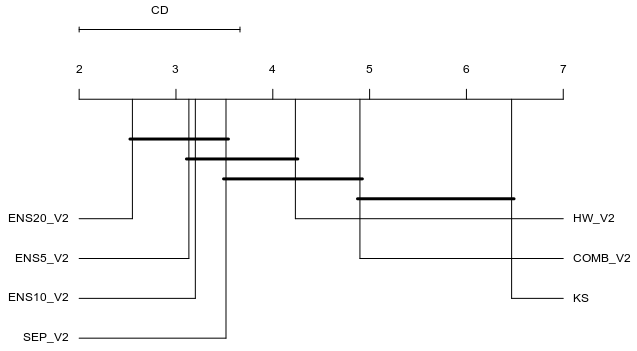
\includegraphics[scale=0.5]{images/mlp_v2_happy.png}
  \caption{Critical difference diagram for MLP using handwriting v1 for ``happy'' emotion}
  \label{fig:cd-happy}
\end{figure}

From Figure \ref{fig:cd-happy}, it can be observed that ENS20 proposed approach presented the best ranking in the CD diagram since it is located in the furthermost left position of the CD diagram. Additionally, this figure shows that there is no horizontal line connecting ENS20 to any individual biometric modality, indicating a statistically significant difference between ENS20 and both individual biometric modalities. These results only confirm the superiority, in terms of accuracy, of the proposed method over individual use, for ``happy'' emotional state. 

\begin{figure}[htbp]
  \centering
  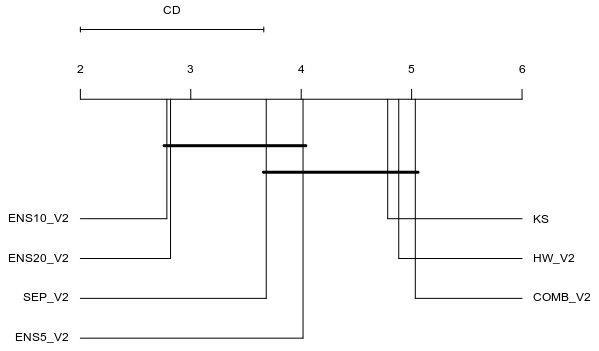
\includegraphics[scale=0.5]{images/mlp_v2_relaxed.png}
  \caption{Critical difference diagram for MLP using handwriting v1 for ``relaxed'' emotion}
  \label{fig:cd-relaxed}
\end{figure}

From Figure \ref{fig:cd-relaxed}, it can be seen that ENS10 and ENS20 proposed approaches also presented
the best rankings in the CD diagram. Also, this figure illustrates that there is no horizontal line connecting ENS10 and ENS20 to any individual biometric modality, indicating, once again, statistically significant differences. Finally, this result depicts that there is a superiority, in terms of performance,  of two combination approaches over individual modalities, for ``relaxed'' emotional state. 


\section{Final Remarks}

This paper presented the results of an initial investigation of how the keystroke and handwriting biometrics modalities combination can impact the prediction accuracy of emotional states. In this sense, two different combination approaches (data fusion and decision fusion) were analyzed. Also, four different classification algorithms ($k$-NN, MLP, DT, and SVM) were assessed to provide a substantial amount of results to be evaluated.

After analyzing the results on ``happy''  and ``relaxed'' emotional states, it is possible to state that combining keystroke and handwriting behavioral modalities generates a substantially positive impact on its prediction accuracy.
Additionally, the statistical tests proved that at least one combination approach outperforms the accuracy delivered by the individual modalities.
Being that said, the results presented in this paper bring a real contribution to the biometrics field. The results may also work as a start point to new researches, especially related to combining behavioral modalities in soft biometrics prediction tasks.

As future works, we intend to explore the impact of dimensionality reduction methods in this task as well as the use of more classifier algorithms. For the second part of the decision fusion approach, we plan to study the use of more complex and elaborated feature selection methods. Besides, the indications of a potential superiority of dynamic handwriting features will be deepen explored.
Finally, we plan to create a new dataset containing more information and more biometric modalities.
 
 
\bibliographystyle{IEEEtran}
\bibliography{IEEEfull, Referencias2}

\end{document}
